\documentclass[sigconf]{acmart}
\usepackage{graphicx} % Required for inserting images
\usepackage{biblatex} %Imports biblatex package
\addbibresource{citations.bib}

\begin{document}
\title{The Two-Tower Recommender System}


\author{Bruno Berndt Lima}
\email{brunolima674@usp.br}
\affiliation{%
  \institution{Universidade de São Paulo - USP}
  \city{São Carlos}
  \state{São Paulo}
  \country{Brasil}
}

\author{Fernando Gonçalves Campos}
\email{fernandogc@usp.br}
\affiliation{%
  \institution{Universidade de São Paulo - USP}
  \city{São Carlos}
  \state{São Paulo}
  \country{Brasil}
}

\begin{teaserfigure}
  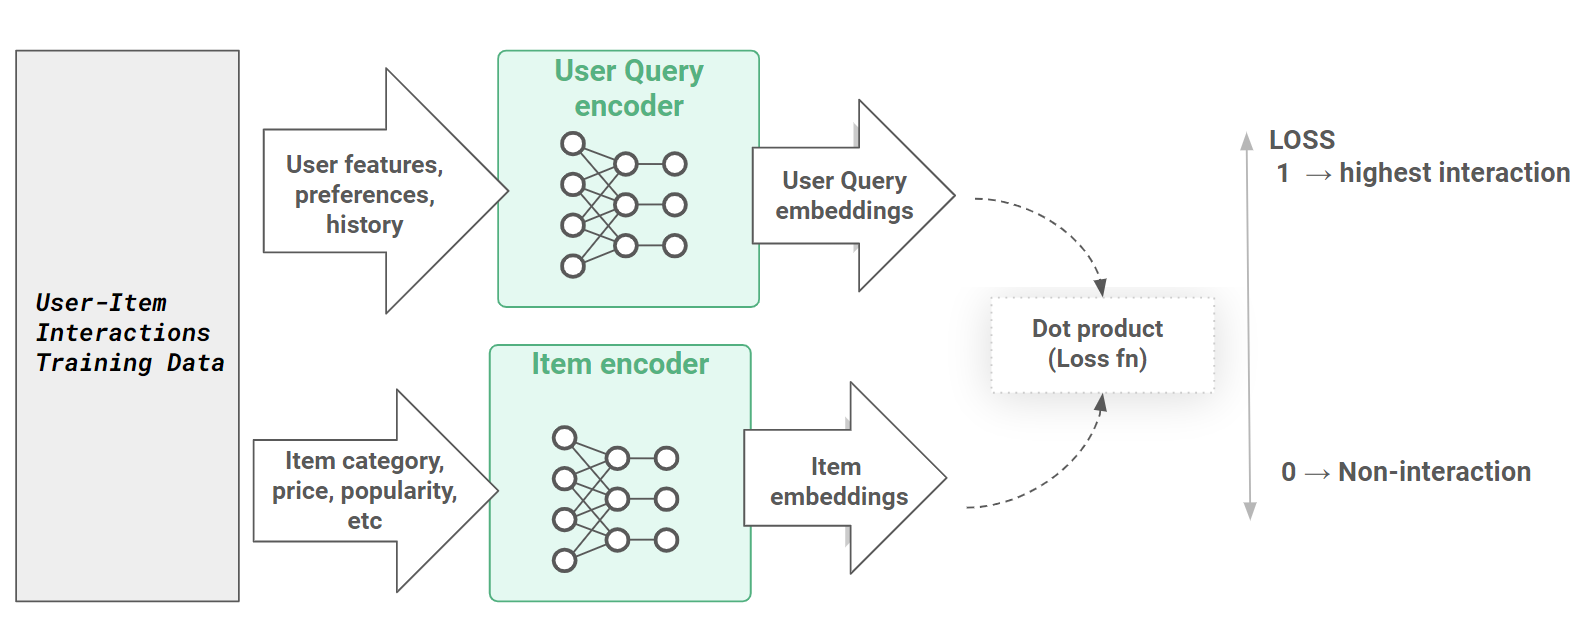
\includegraphics[width=\textwidth]{two_tower_model.png}
  \caption{Two-tower embedding model architecture}
  \label{fig:teaser}
\end{teaserfigure}


\begin{abstract}
  Este artigo apresenta a implementação de um modelo de recomendação conhecido como Two-Tower (Duas Torres), amplamente utilizado para aprimorar sistemas de recomendação personalizados. O modelo baseia-se em redes neurais, com duas torres separadas que aprendem representações independentes de usuários e itens, permitindo a combinação eficiente dessas representações para gerar recomendações mais precisas. Utilizando o dataset \cite{MovieLens}, o modelo é treinado para aprender embeddings vetoriais de usuários e filmes, empregando a similaridade entre essas representações para gerar recomendações personalizadas. O desempenho do modelo Two-Tower é comparado com outras abordagens de recomendação, como KNN e filtragem colaborativa tradicional, demonstrando sua eficácia em melhorar a precisão das recomendações.
\end{abstract}

\keywords{Two-Tower, Sistemas de recomendação, Redes neurais, Embeddings}

\maketitle

\section{Introdução}

Nos últimos anos, os sistemas de recomendação têm se tornado componentes essenciais em diversas plataformas online, como e-commerce, serviços de streaming e redes sociais. Com o crescente volume de dados gerados diariamente, a capacidade de fornecer recomendações personalizadas de forma eficiente e precisa tornou-se um diferencial competitivo. Entre as abordagens mais promissoras para esse desafio, os modelos baseados em aprendizado profundo têm se destacado, oferecendo maior capacidade de capturar padrões complexos de interação entre usuários e itens.

O modelo \textit{Two-Tower} (Duas Torres) é uma dessas abordagens, amplamente utilizado para gerar recomendações personalizadas. Este modelo utiliza duas redes neurais separadas: uma torre dedicada a aprender as características dos usuários, e outra torre dedicada aos itens. Através da combinação dessas representações, o modelo é capaz de calcular a similaridade entre usuários e itens, gerando recomendações mais precisas e relevantes.

Neste trabalho, apresentamos a implementação do modelo \textit{Two-Tower} aplicada ao \textit{dataset} MovieLens, um conjunto de dados amplamente utilizado em pesquisas sobre sistemas de recomendação. Disponibilizado pelo GroupLens Research, ele reúne informações detalhadas sobre avaliações de filmes realizadas por usuários, servindo como referência para estudos e desenvolvimento de algoritmos de recomendação. Além de explorar a arquitetura e o processo de treinamento do modelo, comparamos seu desempenho com uma abordagem tradicional, o KNN, utilizando métricas de avaliação como \textit{MSE}, \textit{RMSE} \textit{Precision@k}, \textit{Recall@k}, \textit{MAP@k}. Também discutimos os benefícios dessa abordagem e suas aplicações em cenários reais.

O restante deste artigo está organizado da seguinte forma: a Seção 2 apresenta o histórico dos sistemas de recomendação, a Seção 3 descreve a arquitetura do modelo \textit{Two-Tower}, a Seção 4 detalha o processo de treinamento e avaliação, e a Seção 5 discute os resultados experimentais e a comparação com outros modelos. Finalmente, a Seção 6 apresenta as conclusões e sugestões para trabalhos futuros.

\section{Histórico dos Sistemas de Recomendação}

Os sistemas de recomendação têm sido amplamente estudados nas últimas décadas, com diferentes abordagens sendo aplicadas para melhorar a qualidade das recomendações. Entre as técnicas tradicionais, a \textit{filtragem colaborativa} destaca-se como uma das mais utilizadas. Ela se baseia no pressuposto de que usuários com preferências similares no passado continuarão a ter gostos semelhantes no futuro. A filtragem colaborativa pode ser dividida em duas categorias: baseada em usuários e baseada em itens. A abordagem baseada em usuários recomenda itens que outros usuários semelhantes gostaram, enquanto a abordagem baseada em itens recomenda itens similares àqueles que o usuário já apreciou. Apesar de sua eficácia, essa técnica enfrenta desafios como o \textit{cold start} e a \textit{esparsidade de dados}, especialmente em plataformas com grandes catálogos de itens.

Outra abordagem relevante é o uso de modelos baseados em \textit{machine learning}, que vão além das heurísticas tradicionais. Modelos como o KNN (K-Nearest Neighbors) e o SVD (Singular Value Decomposition) são amplamente utilizados para encontrar padrões em grandes volumes de dados de interações entre usuários e itens. Esses modelos oferecem maior flexibilidade e precisão, mas também exigem maior capacidade computacional e mais dados para alcançar bons resultados.

Nos últimos anos, o advento das redes neurais introduziu novas formas de modelagem para sistemas de recomendação. Modelos de aprendizado profundo, como o \textit{Neural Collaborative Filtering} (NCF) e \textit{Wide \& Deep}, utilizam redes neurais para capturar representações não lineares de interações entre usuários e itens. Esses modelos são capazes de aprender embeddings mais complexos, representando melhor as preferências dos usuários e as características dos itens, resultando em recomendações mais precisas.

O modelo \textit{Two-Tower}, foco deste trabalho, surge nesse contexto como uma evolução dos modelos de redes neurais aplicados a sistemas de recomendação. Ele adota uma abordagem dual, com uma torre responsável por processar as características dos usuários e outra para os itens. Essa estrutura facilita o aprendizado de representações vetoriais (\textit{embeddings}) independentes para usuários e itens, que são posteriormente combinadas para calcular a similaridade e gerar recomendações personalizadas. A arquitetura \textit{Two-Tower} tem sido utilizada com sucesso em várias plataformas, como Spotify e YouTube, demonstrando sua eficiência em cenários de grande escala.

Portanto, neste trabalho, exploramos como o modelo \textit{Two-Tower} pode ser aplicado ao \textit{dataset} MovieLens, comparando seu desempenho com o KNN. Nossa contribuição inclui a análise do impacto dessa abordagem baseada em redes neurais na precisão e relevância das recomendações personalizadas.

\section{Arquitetura do Modelo Two-Tower}

O modelo \textit{Two-Tower} (Duas Torres) é uma arquitetura de redes neurais amplamente utilizada em sistemas de recomendação devido à sua capacidade de aprender representações independentes para usuários e itens. A principal característica desse modelo é sua estrutura composta por duas redes separadas, ou "torres", uma para o processamento das características dos usuários e outra para os itens. Essas redes são treinadas simultaneamente para gerar \textit{embeddings} que capturam as preferências dos usuários e as características dos itens. A similaridade entre esses \textit{embeddings} é então utilizada para gerar recomendações personalizadas.

\subsection{Estrutura da Torre de Usuários}

A torre dedicada aos usuários é responsável por processar informações relacionadas ao histórico e preferências do usuário. Os dados de entrada para essa torre podem incluir interações anteriores com itens, avaliações fornecidas, categorias de interesse e outras características demográficas. Esses dados são passados por uma rede neural, que geralmente consiste em várias camadas densas (\textit{fully connected layers}), para aprender uma representação vetorial (\textit{embedding}) compacta do usuário.

\subsection{Estrutura da Torre de Itens}

A torre de itens segue uma arquitetura similar à torre de usuários, mas seu objetivo é aprender as representações dos itens (como filmes, no caso do dataset MovieLens). Os dados de entrada podem incluir características do item, como o título, gênero, atores principais, ou até mesmo informações de conteúdo, como descrições textuais ou imagens. Assim como a torre de usuários, a torre de itens gera um \textit{embedding} que captura as características latentes do item. 

\subsection{Combinação das Torres}

Após o treinamento das duas torres, as representações (\textit{embeddings}) geradas para usuários e itens são combinadas para calcular a similaridade entre eles. Um método comum para essa combinação é o produto escalar entre os \textit{embeddings}, que resulta em uma pontuação de relevância. A função de similaridade é dada por:

\begin{equation}
    s(u, i) = h_{u} \cdot h_{i}
\end{equation}

onde $h_{u}$ é o \textit{embedding} do usuário e $h_{i}$ é o \textit{embedding} do item. Essa pontuação é usada para classificar os itens mais relevantes para cada usuário.

\subsection{Benefícios da Arquitetura Two-Tower}

A arquitetura \textit{Two-Tower} oferece uma série de vantagens para sistemas de recomendação em grande escala. Primeiro, sua separação entre as características de usuários e itens permite que as torres sejam treinadas de forma independente, o que é vantajoso para sistemas com muitos usuários e itens. Além disso, o uso de \textit{embeddings} compactos reduz a dimensionalidade dos dados, tornando o modelo mais eficiente em termos de computação e memória. Outro benefício é a flexibilidade de incluir novos dados de entrada, como informações contextuais ou dados multimodais (texto, imagem), que podem ser facilmente incorporados no treinamento das torres.

Por fim, a combinação das duas torres permite que o modelo gere recomendações personalizadas de forma eficiente, mesmo em cenários de grandes volumes de dados, como plataformas de streaming ou comércio eletrônico.

\section{Treinamento e Avaliação}

\subsection{Pré-processamento dos Dados}

O pré-processamento dos dados é uma etapa crucial para preparar o conjunto de dados MovieLens para o treinamento do modelo Two-Tower. Primeiramente, os arquivos contendo as avaliações dos usuários e informações sobre os filmes foram carregados, e apenas as colunas relevantes foram mantidas. Para otimizar o processamento, os IDs de usuários e filmes foram mapeados para índices numéricos contínuos. As avaliações dos filmes, originalmente variando de 1 a 5, foram normalizadas para um intervalo de 0 a 1. Além disso, os gêneros dos filmes, que podem ser múltiplos por item, foram transformados em uma matriz binária, representando a presença ou ausência de cada gênero. Após essas transformações, os dados foram organizados e preparados para o treinamento do modelo.

\subsection{Treinamento do Modelo}

O modelo Two-Tower foi treinado utilizando otimização por gradiente descendente, com o otimizador Adam, um algoritmo eficiente para redes neurais que ajusta os pesos do modelo para minimizar a função de perda. A função de perda escolhida foi a entropia cruzada binária, que é comumente usada em problemas de recomendação binária. Nesse caso, ela mede a discrepância entre as predições feitas pelo modelo (probabilidade de interação entre usuário e item) e as avaliações reais dos usuários.

A arquitetura do modelo é composta por duas redes neurais independentes, uma para os usuários e outra para os itens. Ambas as redes são formadas por camadas densas com funções de ativação ReLU, o que permite ao modelo capturar não linearidades nas preferências dos usuários e nas características dos itens. As camadas finais de cada rede produzem embeddings vetoriais de dimensão \(d\), que representam de forma compacta as preferências dos usuários e as características dos itens. Esses embeddings são combinados utilizando o produto escalar para calcular a similaridade entre o usuário e o item, gerando as predições de recomendação.

O treinamento é realizado iterativamente por um número pré-determinado de épocas (N\_EPOCHS). Em cada iteração, as representações dos usuários, itens e gêneros são alimentadas ao modelo, e o erro entre as predições do modelo e as avaliações reais é calculado e retropropagado. Esse processo ajusta os pesos das redes neurais para reduzir o erro de predição, aumentando a precisão do modelo ao longo das épocas. A taxa de aprendizado do otimizador Adam é ajustada para otimizar a convergência.

Durante o treinamento, a função de perda é monitorada, e ao final de cada época, o modelo é avaliado para verificar a redução do erro. Caso o treinamento seja interrompido ou o modelo já tenha sido treinado anteriormente, o modelo treinado é salvo e carregado para ser utilizado posteriormente sem a necessidade de reprocessamento.

O modelo é otimizado até que a convergência seja alcançada, ou até que o número máximo de épocas seja atingido.

\subsection{Avaliação do Modelo}

Para avaliar o desempenho do modelo, foram utilizadas métricas comumente empregadas em sistemas de recomendação. A avaliação foi realizada utilizando os dados de teste, onde o modelo previu as classificações para os itens e esses resultados foram comparados com as classificações reais atribuídas pelos usuários. As principais métricas utilizadas foram:

\begin{itemize}
    \item \textbf{MSE (Erro Quadrático Médio)}: Mede a média dos quadrados das diferenças entre as previsões do modelo e as classificações reais. Essa métrica penaliza grandes erros de forma quadrática, proporcionando uma visão geral da precisão das previsões do modelo.
    
    \item \textbf{RMSE (Raiz do Erro Quadrático Médio)}: Calcula a raiz quadrada do MSE, tornando a unidade da métrica equivalente à dos dados originais, o que facilita a interpretação do erro médio do modelo.
    
    \item \textbf{\( R^2 \) (Coeficiente de Determinação)}: Mede a proporção da variabilidade total das classificações que é explicada pelo modelo. Um valor de \( R^2 \) próximo de 1 indica que o modelo explica bem os dados, enquanto valores próximos de 0 indicam um desempenho ruim.
    
    \item \textbf{Precision@k}: Avalia a precisão das \(k\) primeiras recomendações fornecidas pelo modelo. Essa métrica indica a proporção de itens relevantes entre as \(k\) recomendações feitas.
    
    \item \textbf{Recall@k}: Mede a capacidade do modelo de recuperar itens relevantes entre as \(k\) primeiras recomendações. Indica a quantidade de itens relevantes que foram realmente recomendados.
    
    \item \textbf{MAP@k (Média da Precisão em \(k\))}: Calcula a média da precisão acumulada nas \(k\) primeiras recomendações, levando em conta a ordem de relevância dos itens recomendados. A MAP@k proporciona uma visão mais detalhada sobre a qualidade das recomendações em termos de relevância para o usuário.
\end{itemize}

O modelo foi avaliado utilizando os dados de teste e as métricas foram calculadas para fornecer uma visão precisa do seu desempenho.

\subsection{Comparação com Outros Modelos}

Além de avaliar o desempenho do modelo Two-Tower isoladamente, também realizamos uma comparação com o o UserKNN. Utilizamos as mesmas métricas de avaliação para garantir uma comparação justa entre os modelos. 

\section{Resultados e Discussão}

Os experimentos realizados permitiram comparar o desempenho do modelo Two-Tower proposto com o baseline UserKNN em tarefas de recomendação. A avaliação foi realizada utilizando métricas tradicionais mencionadas anteriormente para diferentes tamanhos de lista de recomendação (k=5, 10 e 20).

Os resultados demonstram que o UserKNN apresentou performance superior ao modelo Two-Tower em todas as métricas avaliadas. Para k=5, o UserKNN alcançou Precision de 0.253, Recall de 0.368 e MAP de 0.515, enquanto o Two-Tower obteve valores de 0.058, 0.084 e 0.161 respectivamente. Esta tendência se manteve para k=10 e k=20.

Um aspecto notável é o comportamento do Recall à medida que k aumenta. O UserKNN apresentou um crescimento significativo no Recall, atingindo 0.705 para k=20, indicando uma boa capacidade de recuperação de itens relevantes. Em contraste, o Two-Tower demonstrou um crescimento mais modesto, alcançando apenas 0.172 de Recall para k=20.

A diferença expressiva de desempenho pode ser atribuída a alguns fatores:

1. O UserKNN trabalha diretamente com as interações usuário-item, enquanto no Two-Tower foram utilizadas embeddings gerados via PCA, que podem perder informações relevantes no processo de redução dimensional.

2. A arquitetura neural do Two-Tower, apesar de sua capacidade de aprender representações complexas, pode ter sido limitada pelo tamanho do conjunto de dados ou pela escolha de hiperparâmetros.

3. O UserKNN é particularmente eficaz em cenários de recomendação onde a similaridade entre usuários é um forte indicador de preferências, que parece ser o caso neste conjunto de dados.

\section{Conclusão}

Embora os resultados experimentais tenham demonstrado uma performance inferior do modelo Two-Tower em comparação ao UserKNN neste contexto específico, é fundamental ressaltar a importância e as vantagens que as arquiteturas neurais, como o Two-Tower, trazem para o campo dos sistemas de recomendação.

O Two-Tower apresenta características cruciais para aplicações em larga escala, como:

\textbf{1. Escalabilidade}: Diferentemente do UserKNN, que requer o cálculo de similaridades entre todos os usuários em tempo real, o Two-Tower permite inferências rápidas uma vez treinado, tornando-o mais adequado para sistemas com milhões de usuários e itens.

\textbf{2. Flexibilidade}: A arquitetura neural possibilita a incorporação de diferentes tipos de features e modalidades de dados (texto, imagem, áudio), permitindo recomendações mais ricas e contextualizadas. Um exemplo de flexibilidade é a adição de features para medir os interesses recentes do usuário, que podem ser gerados a partir de uma RNN que é sendo atualizada depois de cada avaliação, por exemplo. Enquanto uma rede neural pode aprender quanto peso dar para cada tipo de dado, o KNN pode precisar da escolha dos pesos de forma manual.

\textbf{3. Aprendizado Contínuo}: O modelo pode ser facilmente atualizado com novos dados, adaptando-se a mudanças no comportamento dos usuários e à introdução de novos itens.

\textbf{4. Eficiência Computacional}: Os embeddings gerados podem ser pré-computados e armazenados, permitindo recomendações em tempo real mesmo em grandes conjuntos de dados.

Além disso, há diversos caminhos para potencial melhoria do modelo Two-Tower, como a exploração de diferentes arquiteturas de rede, técnicas de regularização mais sofisticadas e estratégias de geração de embeddings de entrada mais robustas. O modelo também poderia se beneficiar de um conjunto de dados maior e mais diversificado para treinamento.

Portanto, apesar dos resultados comparativos neste estudo específico, o Two-Tower permanece como uma abordagem promissora e relevante no campo dos sistemas de recomendação, especialmente em cenários que demandam escalabilidade e flexibilidade.

\section{Avaliação do público alvo}

A avaliação será feita através de um formulário. Foi perguntado: 

\begin{enumerate}
    \item A explicação do conteúdo foi clara e fácil de entender?
    \item Algum comentário que gostaria de fazer sobre a qualidade da explicação?
    \item A aula despertou seu interesse sobre o assunto?
    \item Existe algo que você acredita que faltou ser abordado na aula?
    \item O assunto abordado foi relevante o seu dia a dia?
    \item Você se sente motivado a pesquisar mais sobre o assunto?
    \item Qual a sua opinião sobre a duração da aula em relação ao que foi abordado?
    \item Gostaria de adicionar algum comentário sobre a aula?
\end{enumerate}

\section{Recursos adicionais}

Links para o que foi realizado no trabalho

\href{https://github.com/Fernando-Goncalves-Campos/Two-Tower-Recommender-Systems}{Código}

\href{https://drive.google.com/file/d/1NcdgdX3pl0ckHoycoLXk8ErormbaWQan/view?usp=sharing}{Aula}

\href{https://docs.google.com/forms/d/e/1FAIpQLSfs23afuEESuf2PkeNfgvy1k7LwaSePt5ZhKzjw_IRcuJCAgA/viewform?usp=sharing}{Formulário}


\printbibliography[title={Referências}]

\end{document}
